\section{Introduction}

This chapter applies the methods of \eqref{chap:dist-opt} and \eqref{chapt:cs-inference} to real-world datasets. One is provided by OFCOM, the other captured as part of the PhD work. The captured dataset was captured by an RTL-SDR. Both datasets are of the TVWS band 440-780MHz. The OFCOM datset was taken in Southwark, UK during May 2014, whilst the other dataset was captured during July 2016, in Bristol, UK. 

This chapter is organised as follows: we first show results, on both datasets, of the distributed estimation algorithm (presented in chapter \eqref{chap:dist-opt}, with estimation in the Heavyside basis. We do so for the LASSO and MMV-LASSO variations of the alogorithm.

We then present results of the techineques outlined in chapter \eqref{chap:cs-inference} on both datasets.

\section{Data Set}

\section{Results: Distributed Estimation with Heaviside Basis}

\begin{figure}[h]
\centering
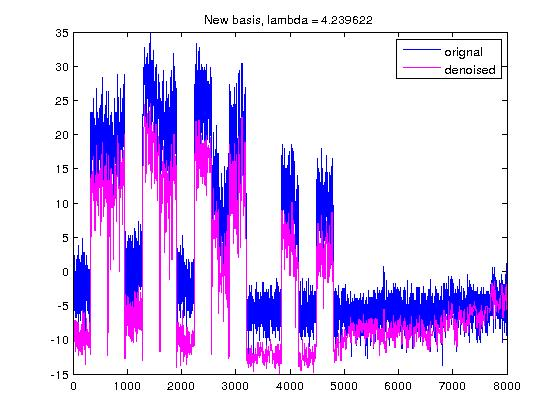
\includegraphics[height = 7.3 cm]{new_basis_ofcom_1.jpg}
\caption{Example of classification with OFCOM data, 35 changepoints}
\label{fig:hvb}
\end{figure}

\begin{figure}[h]
\centering
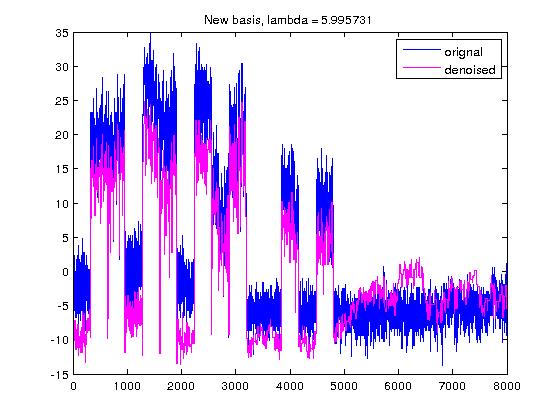
\includegraphics[height = 7.3 cm]{new_basis_ofcom_2.jpg}
\caption{Example of classification with OFCOM data, 55 changepoints}
\label{fig:hvb}
\end{figure}

\begin{figure}[h]
\centering
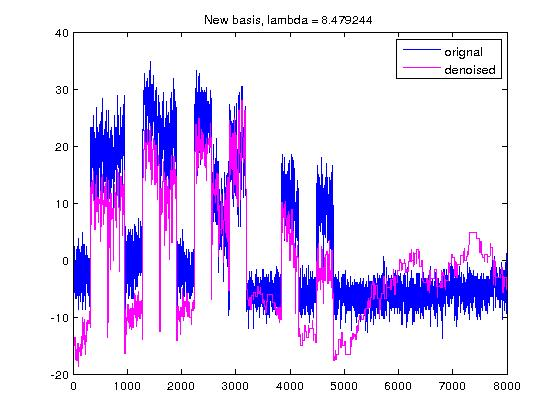
\includegraphics[height = 7.3 cm]{new_basis_ofcom_3.jpg}
\caption{Example of classification with OFCOM data, 35 changepoints}
\label{fig:hvb}
\end{figure}

\begin{figure}[h]
\centering
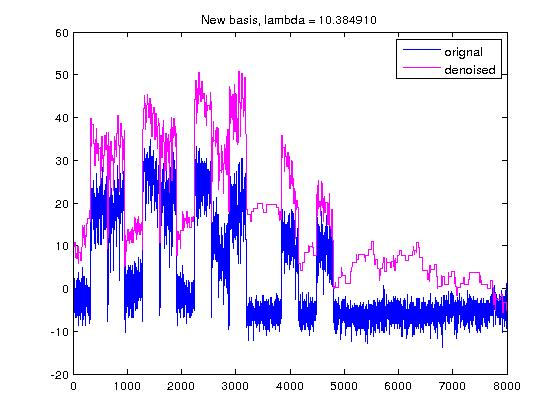
\includegraphics[height = 7.3 cm]{new_basis_ofcom_4.jpg}
\caption{Example of classification with OFCOM data, 55 changepoints}
\label{fig:hvb}
\end{figure}


\section{Compressive Estimation}

Some examples of the output of this procedure are shown below, for synthetic and real (Ofcom) data.

\begin{figure}[h]
\centering
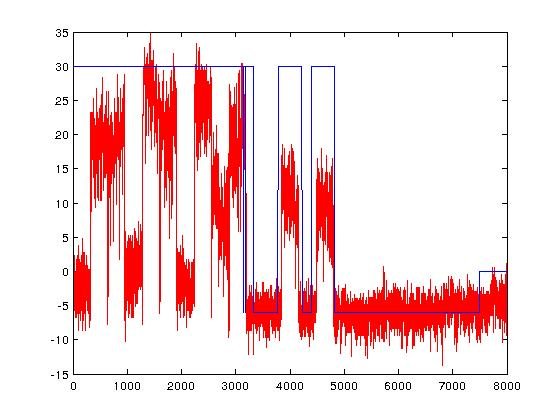
\includegraphics[height = 7.3 cm]{ofcom_classification1.jpg}
\caption{Example of classification with OFCOM data, 35 changepoints}
\label{fig:hvb}
\end{figure}

\begin{figure}[h]
\centering
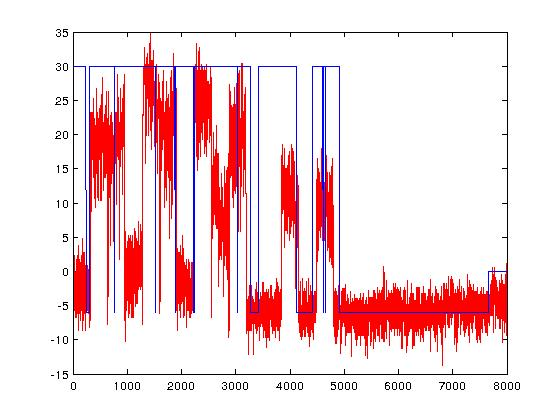
\includegraphics[height = 7.3 cm]{ofcom_classification.jpg}
\caption{Example of classification with OFCOM data, 55 changepoints}
\label{fig:hvb}
\end{figure}

\begin{figure}[h]
\centering
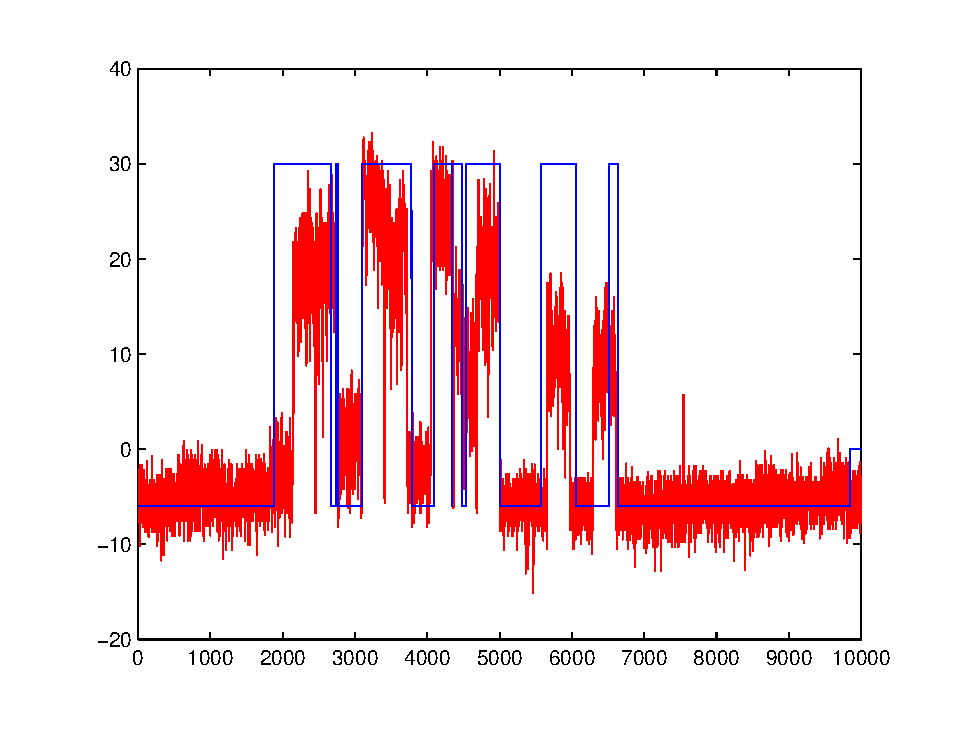
\includegraphics[height = 7.3 cm]{OFCOM5.eps}
\caption{Example of classification with OFCOM data, 35 changepoints}
\label{fig:hvb}
\end{figure}

\begin{figure}[h]
\centering
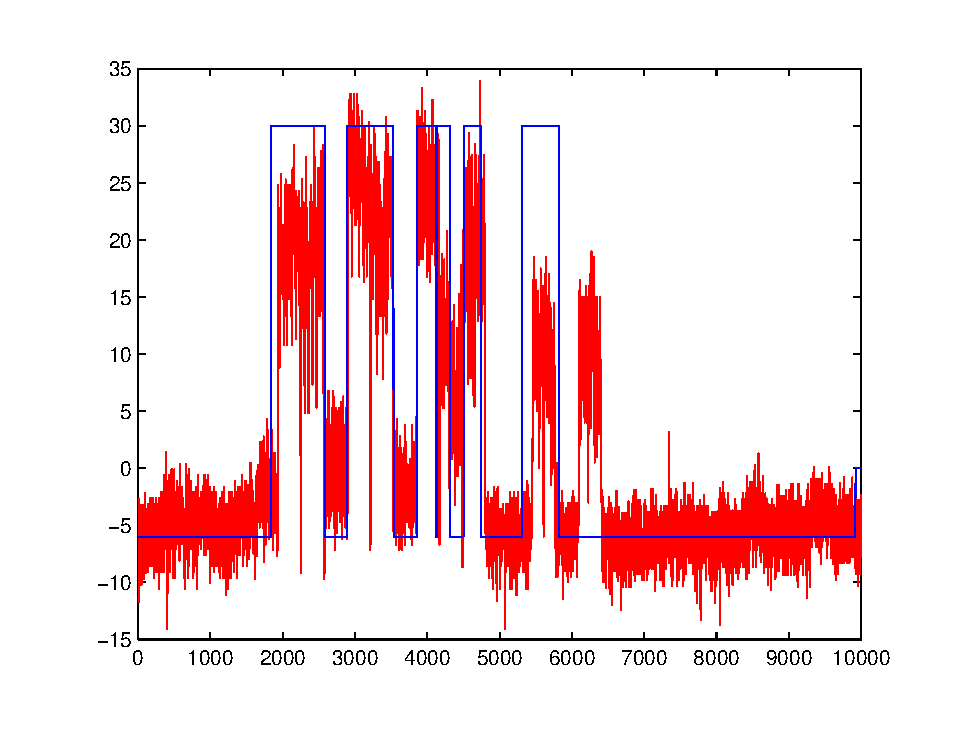
\includegraphics[height = 7.3 cm]{OFCOM6.eps}
\caption{Example of classification with OFCOM data, 55 changepoints}
\label{fig:hvb}
\end{figure}

\begin{figure}[h]
\centering
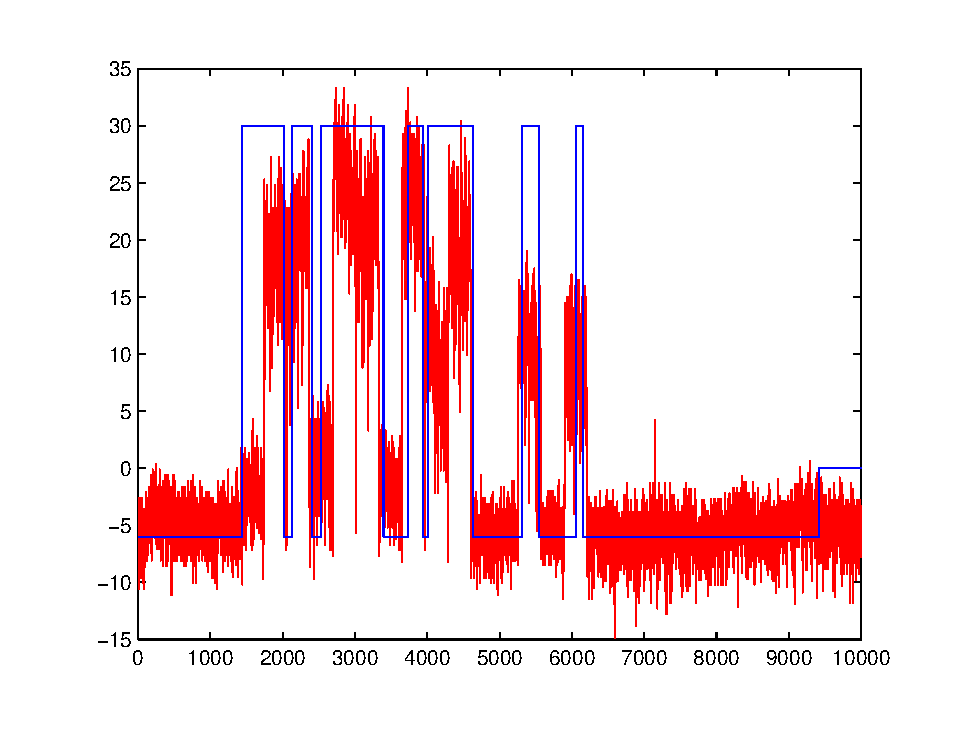
\includegraphics[height = 7.3 cm]{OFCOM7.eps}
\caption{Example of classification with OFCOM data, 35 changepoints}
\label{fig:hvb}
\end{figure}

\begin{figure}[h]
\centering
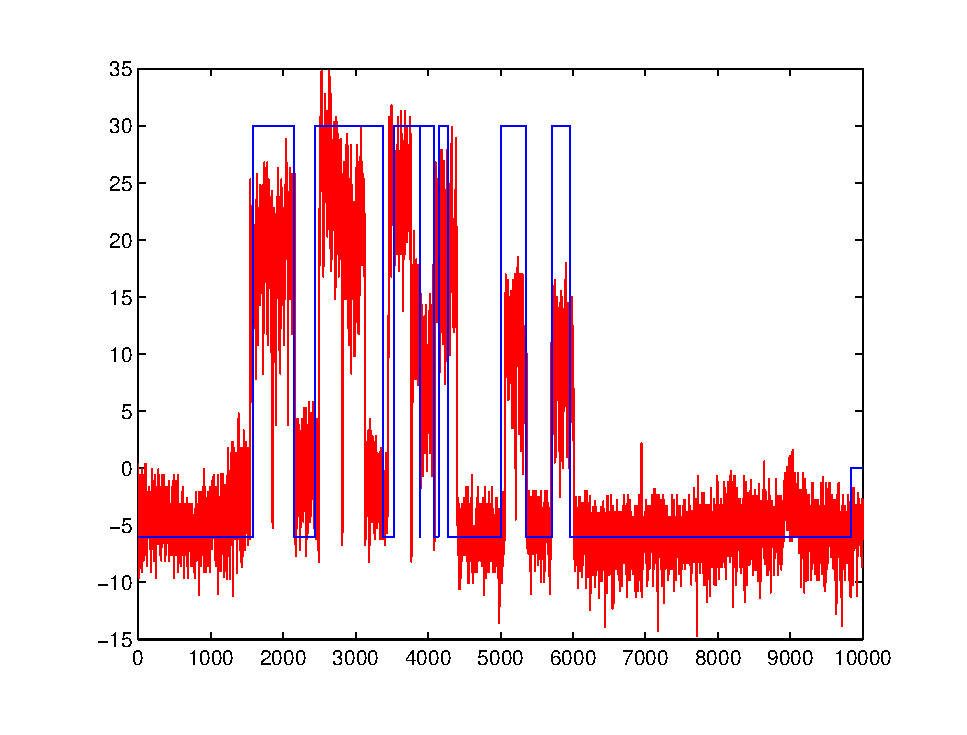
\includegraphics[height = 7.3 cm]{OFCOM8.eps}
\caption{Example of classification with OFCOM data, 55 changepoints}
\label{fig:hvb}
\end{figure}
